\documentclass[reprint,amsmath,amssymb,aps]{revtex4-2}

\usepackage[utf8]{inputenc}
\usepackage[T1]{fontenc}
\usepackage{physics}
\usepackage{graphicx}
\usepackage{dcolumn}
\usepackage{multirow}
\usepackage{booktabs}
\usepackage{float}
\usepackage{bm}
\usepackage{makecell}
\usepackage{siunitx}
\usepackage{hyperref}

\begin{document}
	
	\title{Lagrange Interpolation and Classical Numerical Integration Applied to the Analysis of Orbital Trajectories}
	
	\author{Juan Carlos Celis Lozada}
	\email[]{juan.celisloz@unipamplona.edu.co}
	\affiliation{Universidad de Pamplona, Physics Program, Pamplona, Norte de Santander, Colombia}
	
	\date{\today}
	
	\begin{abstract}
		Polynomial interpolation is a fundamental tool in numerical analysis for reconstructing functions from discrete data, with direct applications to physical and astrodynamical problems. In this work, the performance of Lagrange polynomial interpolation applied to elliptical orbital trajectories described by a Keplerian expression is analyzed. A computational procedure implemented in Python is used to sample the orbit, reconstruct it using a global interpolating polynomial, and quantify the geometric error as a function of the number of nodes and the orbital eccentricity. Furthermore, the impact of interpolation on subsequent numerical integration calculations is evaluated by comparing the values of the radial integral obtained from the analytical orbit and from the interpolated orbit using Simpson's rule and Gauss--Legendre quadrature. The results show that the accuracy of the interpolation depends critically on the discretization and the orbital geometry, with oscillations associated with the Runge phenomenon becoming evident for equally spaced meshes. Despite this, the numerical integrals computed from the interpolated function exhibit relative discrepancies below $0.1\%$, highlighting the robustness of quadrature methods with respect to moderate errors in the input function.
	\end{abstract}
	
	\keywords{Lagrange interpolation; Polynomial approximation; Orbital trajectories; Numerical error; Simpson integration; Gauss--Legendre quadrature}
	
	\maketitle
	
	\section{Introduction}
	
	Function interpolation is a fundamental procedure in numerical analysis, used to approximate an unknown function from a finite set of experimental or computed data. Its applications span a wide range of scientific and engineering problems, including signal processing, numerical solutions of differential equations, and the reconstruction of physical trajectories from discrete measurements \cite{BurdenFaires,Atkinson}.
	
	Among the different interpolation techniques, polynomial interpolation occupies a central place due to its analytical simplicity and its role in the theoretical development of approximation methods. In particular, the Lagrange interpolation method provides an explicit construction of a unique polynomial of degree at most $n$ that passes exactly through a set of $n+1$ distinct data points \cite{BurdenFaires}. This formulation allows for a direct analytical treatment and serves as a foundation for understanding more advanced interpolation schemes.
	
	Despite its conceptual elegance, global polynomial interpolation is known to exhibit significant limitations. One of the most notable issues is the growth of oscillations near the boundaries of the interpolation interval when equally spaced nodes are used, a behavior commonly referred to as the Runge phenomenon \cite{Runge1901}. This effect leads to large interpolation errors even for smooth functions and has been extensively studied within the framework of approximation theory \cite{Trefethen2013}.
	
	From a practical standpoint, these limitations motivate a careful analysis of the conditions under which Lagrange interpolation can be reliably applied. The choice of node distribution, the degree of the interpolating polynomial, and the nature of the underlying function all play a crucial role in determining the accuracy and stability of the approximation \cite{Atkinson,Trefethen2013}.
	
	In this work, Lagrange polynomial interpolation is applied to the reconstruction of elliptical orbital trajectories described by a Keplerian model. This physical system provides a clear and analytically well-defined reference, making it suitable for evaluating interpolation errors in both geometric and numerical contexts. In addition to analyzing the reconstruction accuracy of the orbit itself, the impact of interpolation errors on subsequent numerical integration procedures is investigated, with particular emphasis on Simpson's rule and Gauss--Legendre quadrature \cite{NumericalRecipes}.
	
	
	\section{Computational Details}
	
	The numerical study presented in this work is based on a set of routines implemented in the Python programming language. The objective of these routines is to analyze the behavior of Lagrange polynomial interpolation when applied to orbital trajectories and to assess its influence on subsequent numerical integration procedures. The computational strategy follows a sequential structure, beginning with the definition of an analytical reference orbit and progressing toward interpolated reconstruction, geometric error evaluation, and numerical quadrature.
	
	The reference orbit is defined using the Keplerian expression for an elliptical trajectory in polar coordinates,
	\begin{equation}
		r(\theta)=\frac{a\left(1-e^{2}\right)}{1-e\cos\theta},
		\label{eq:kepler}
	\end{equation}
	where $a$ denotes the semi-major axis and $e$ the orbital eccentricity. The Cartesian coordinates of the orbit are obtained through the standard polar-to-Cartesian transformations,
	\begin{align}
		x(\theta) &= r(\theta)\cos\theta, \label{eq:xcoord} \\
		y(\theta) &= r(\theta)\sin\theta. \label{eq:ycoord}
	\end{align}
	
	A dense angular grid in the interval $[0,2\pi]$ is used to generate a high-resolution representation of the analytical orbit. This reference solution is treated as the exact trajectory for the purpose of evaluating interpolation and integration errors.
	
	The discrete sampling of the orbit is performed by selecting a finite number $N$ of equally spaced nodes in the angular variable $\theta$. The parameter $N$ is explicitly varied in order to analyze its effect on the accuracy of the interpolated reconstruction. For each choice of $N$, the corresponding sampled points are used as input data for the interpolation procedure.
	
	The interpolating function is constructed using the global Lagrange polynomial. For a generic function $f(\theta)$ sampled at nodes $\theta_i$, the interpolating polynomial is given by
	\begin{equation}
		P(\theta)=\sum_{i=0}^{N-1} f(\theta_i)\,\ell_i(\theta),
		\label{eq:lagrange_poly}
	\end{equation}
	where the Lagrange basis polynomials $\ell_i(\theta)$ are defined as
	\begin{equation}
		\ell_i(\theta)=\prod_{\substack{j=0 \\ j\neq i}}^{N-1}
		\frac{\theta-\theta_j}{\theta_i-\theta_j}.
		\label{eq:lagrange_basis}
	\end{equation}
	
	To quantify the interpolation accuracy, the geometric error is computed as the Euclidean distance between the interpolated trajectory and the analytical reference,
	\begin{equation}
		\varepsilon(\theta)=\sqrt{
			\left[x_{\text{interp}}(\theta)-x_{\text{ref}}(\theta)\right]^2+
			\left[y_{\text{interp}}(\theta)-y_{\text{ref}}(\theta)\right]^2}.
		\label{eq:error}
	\end{equation}
	To evaluate the impact of interpolation on numerical integration procedures, the radial integral
	\begin{equation}
		I=\int_{0}^{2\pi} r(\theta)\,d\theta,
		\label{eq:integral}
	\end{equation}
	is considered. This integral is computed both using the analytical expression given in Eq.~\eqref{eq:kepler} and using the interpolated reconstruction of the orbit. The numerical evaluation of Eq.~\eqref{eq:integral} is performed using the composite Simpson rule and Gauss--Legendre quadrature of finite order, allowing a direct comparison between analytical and interpolated results.
	
	\section{Results}
	
	The Lagrange polynomial interpolation defined in Eq.~\eqref{eq:lagrange_poly} was applied to the Keplerian orbit described by Eq.~\eqref{eq:kepler}. Figure~\ref{fig:orbita5} shows the orbital reconstruction obtained using a small number of interpolation nodes ($N=5$). In this case, significant deviations from the analytical trajectory are observed, particularly in regions where the curvature of the orbit is more pronounced.
	
	As the number of nodes increases, the quality of the interpolation improves substantially, as illustrated in Fig.~\ref{fig:orbita25}. The interpolated trajectory closely follows the analytical orbit over most of the angular domain. However, the Euclidean error profile reveals oscillatory behavior near the boundaries of the interval, which is characteristic of the Runge phenomenon, as shown in Fig.~\ref{fig:error25}.
	
	\begin{figure}[H]
		\centering
		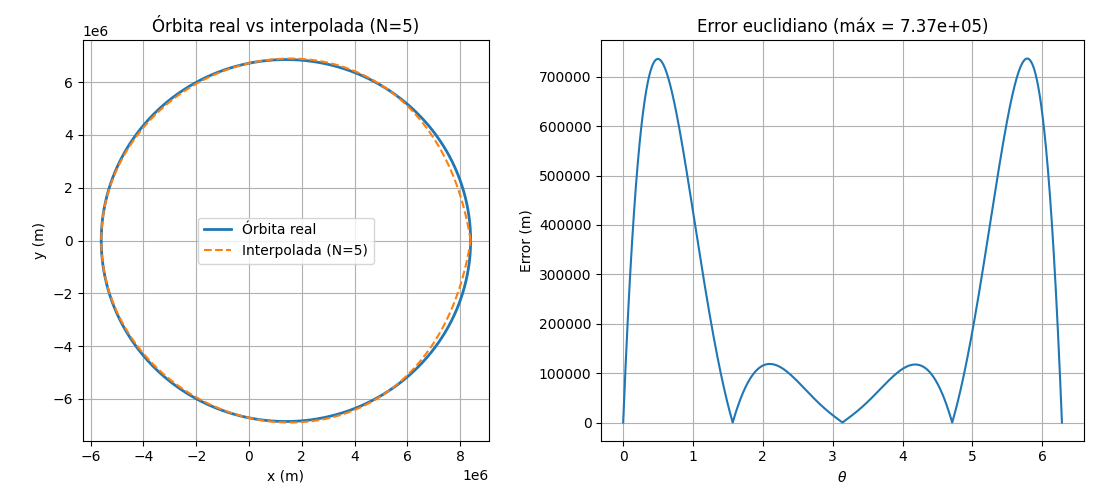
\includegraphics[width=0.45\textwidth]{resultado1.png}
		\caption{Analytical and interpolated orbit (left) and Euclidean error (right) for $N=5$ interpolation nodes.}
		\label{fig:orbita5}
	\end{figure}
	
	\begin{figure}[H]
		\centering
		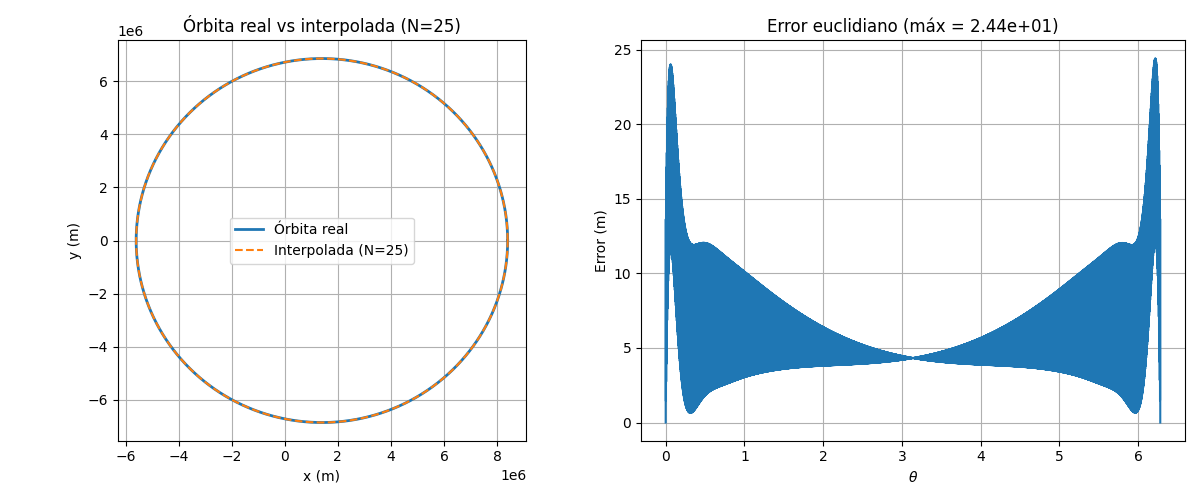
\includegraphics[width=0.45\textwidth]{resultado11.png}
		\caption{Analytical and interpolated orbit (left) and Euclidean error (right) for $N=25$ interpolation nodes.}
		\label{fig:orbita25}
	\end{figure}
	
	\begin{figure}[H]
		\centering
		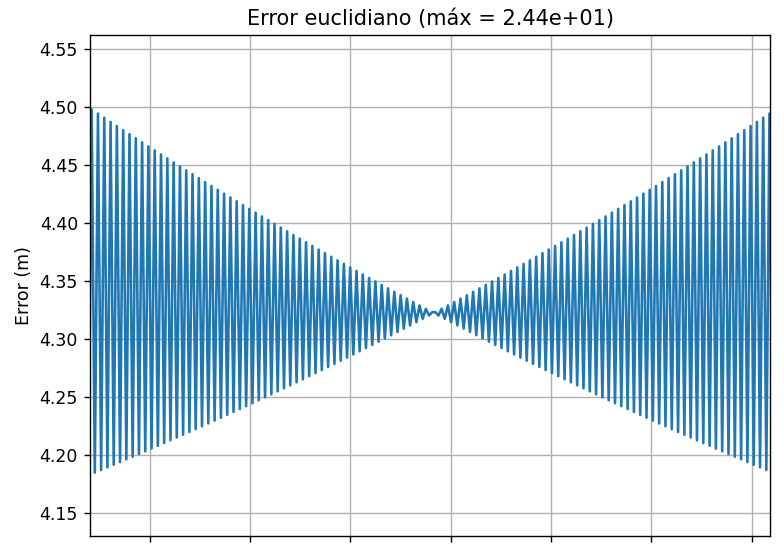
\includegraphics[width=0.45\textwidth]{runge.png}
		\caption{Oscillations in the Euclidean error associated with the Runge phenomenon for $N=25$ nodes.}
		\label{fig:error25}
	\end{figure}
	
	The influence of orbital eccentricity on interpolation accuracy is illustrated in Fig.~\ref{fig:excentricidades}. For a fixed number of nodes ($N=15$), an increase in eccentricity leads to a systematic growth of the interpolation error. This effect becomes particularly pronounced for highly eccentric orbits, where the radial variation near periapsis is more abrupt.
	
	\begin{figure}[H]
		\centering
		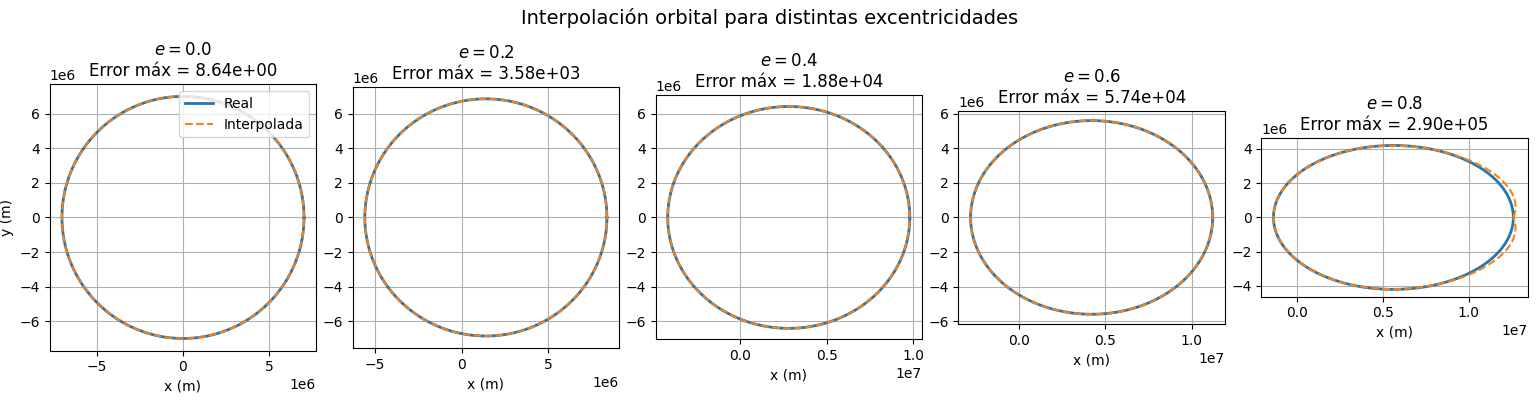
\includegraphics[width=0.45\textwidth]{Excentricidad.png}
		\caption{Analytical and interpolated orbits for different eccentricities using $N=15$ nodes.}
		\label{fig:excentricidades}
	\end{figure}
	
	For the case of high eccentricity ($e=0.8$), the dependence of the interpolation accuracy on the number of nodes is shown in Fig.~\ref{fig:elipticasnodos}. The results indicate that an insufficient number of nodes leads to large geometric errors, while a sufficiently dense discretization allows for an accurate reconstruction of the orbital geometry.
	
	\begin{figure}[H]
		\centering
		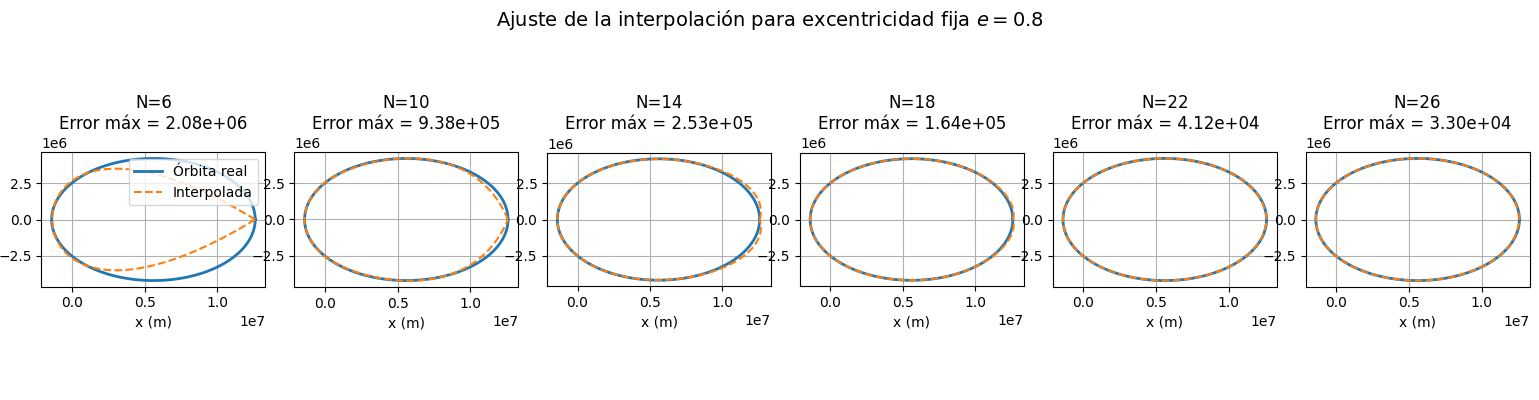
\includegraphics[width=0.45\textwidth]{excentricidad nodos.png}
		\caption{Analytical and interpolated orbits for $e=0.8$ and different numbers of interpolation nodes.}
		\label{fig:elipticasnodos}
	\end{figure}
	
	Table~\ref{tab:integracion} presents a comparison between the radial integral defined in Eq.~\eqref{eq:integral}, evaluated using the analytical orbit and the interpolated orbit. For both numerical integration methods, the absolute differences remain of the order of $10^{4}$, corresponding to relative errors below $0.1\%$.
	
	\begin{table}[H]
		\centering
		\begin{tabular}{ccccc}
			\toprule
			Method & \makecell{Analytical\\Integral} & \makecell{Interpolated\\Integral} & Difference & Error (\%) \\
			\midrule
			Simpson & $2.6389\times 10^{7}$ & $2.6403\times 10^{7}$ & $1.3857\times 10^{4}$ & 0.054 \\
			\makecell{Gauss--\\Legendre} & $2.6359\times 10^{7}$ & $2.6383\times 10^{7}$ & $2.4636\times 10^{4}$ & 0.091 \\
			\bottomrule
		\end{tabular}
		\caption{Comparison between the radial integral computed from the analytical orbit and from the interpolated orbit using Simpson's rule and Gauss--Legendre quadrature.}
		\label{tab:integracion}
	\end{table}
	
	\section{Conclusions}
	In this work, Lagrange polynomial interpolation was analyzed in the context of elliptical orbital trajectories, with particular emphasis on its geometric accuracy and its impact on subsequent numerical integration procedures. The results demonstrate that the quality of the interpolated reconstruction depends critically on both the number of interpolation nodes and the orbital eccentricity.
	
	For coarse discretizations, the geometric error is significant and exhibits oscillatory behavior characteristic of the Runge phenomenon. Increasing the number of nodes leads to a more stable and accurate approximation of the orbital trajectory, provided that the discretization is sufficiently dense to capture the rapid radial variations near periapsis.
	
	The influence of orbital eccentricity was shown to be substantial. As the eccentricity increases, the performance of global polynomial interpolation deteriorates, especially in regions where the orbital geometry changes abruptly. For highly eccentric orbits, careful selection of the number of interpolation nodes is therefore essential to ensure reliable reconstruction.
	
	Regarding numerical integration, the radial integrals computed using the interpolated orbit exhibit only a small systematic bias relative to the analytical solution. Both the composite Simpson rule and Gauss--Legendre quadrature yield relative errors below $0.1\%$, indicating that these quadrature methods are robust against moderate interpolation errors in the input function.
	
	Overall, the results confirm that Lagrange interpolation can be effectively employed in astrodynamical applications, provided that appropriate attention is given to node distribution and orbital geometry. The study also highlights the importance of balancing interpolation accuracy with computational efficiency when applying global polynomial methods to physically relevant problems.
	
	\begin{thebibliography}{99}
		
		\bibitem{BurdenFaires}
		R. L. Burden and J. D. Faires,
		\textit{Numerical Analysis},
		Cengage Learning (2011).
		
		\bibitem{Atkinson}
		K. Atkinson,
		\textit{An Introduction to Numerical Analysis},
		Wiley (1989).
		
		\bibitem{Runge1901}
		C. Runge,
		``On empirical functions and interpolation between equidistant ordinates,''
		Zeitschrift für Mathematik und Physik \textbf{46}, 224--243 (1901).
		
		\bibitem{Trefethen2013}
		L. N. Trefethen,
		\textit{Approximation Theory and Approximation Practice},
		SIAM (2013).
		
		\bibitem{NumericalRecipes}
		W. Press, S. Teukolsky, W. Vetterling, and B. Flannery,
		\textit{Numerical Recipes},
		Cambridge University Press (2007).
		
	\end{thebibliography}
	\section*{Appendix}
	
	\begin{figure}[H]
		\centering
		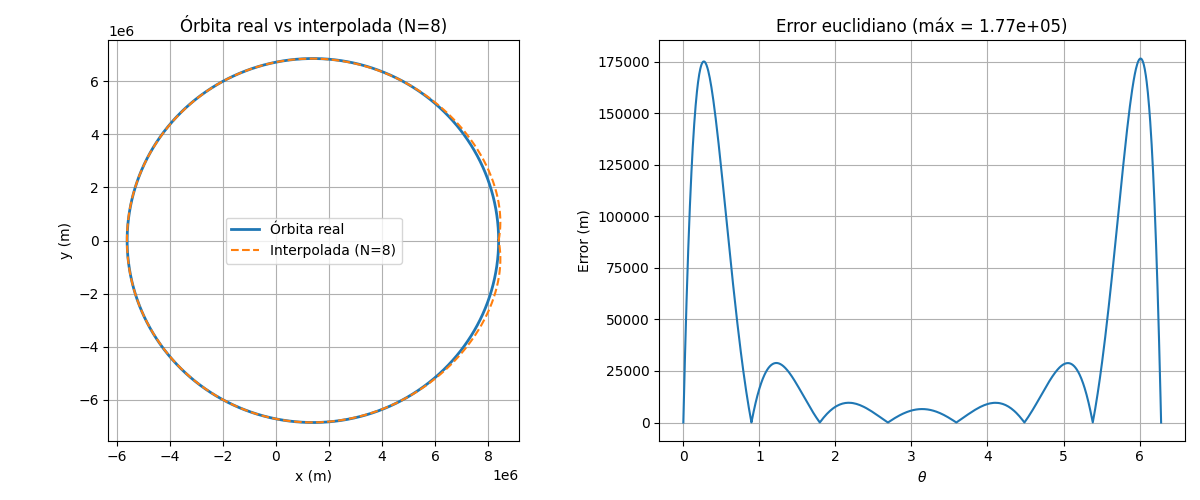
\includegraphics[width=0.5\textwidth]{resultado3.png}
		\caption{Analytical and interpolated orbit (left) and corresponding Euclidean error (right) for $N=8$ interpolation nodes.}
		\label{fig:orbita8}
	\end{figure}
	
	\begin{figure}[H]
		\centering
		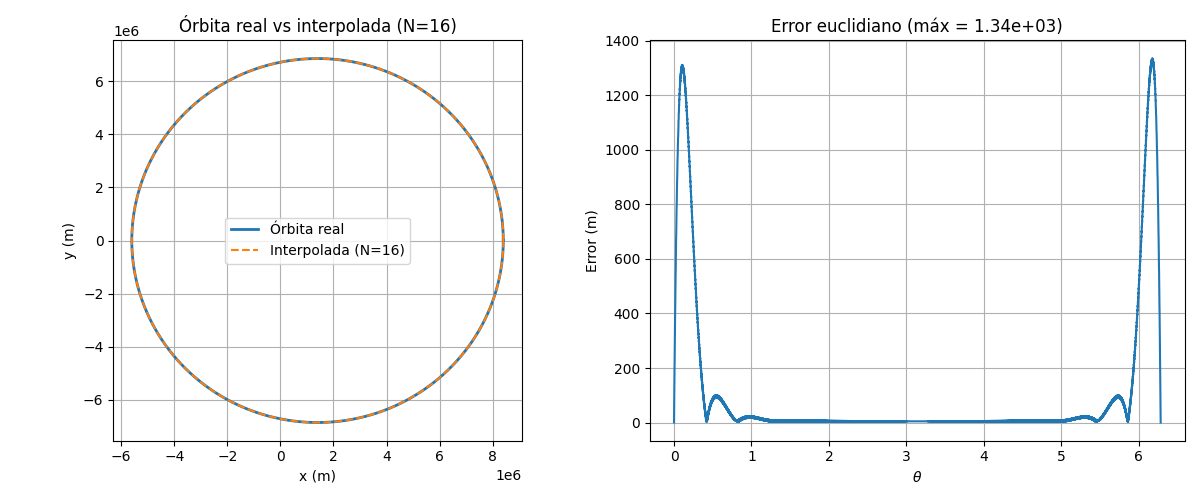
\includegraphics[width=0.5\textwidth]{resultado7.png}
		\caption{Analytical and interpolated orbit (left) and corresponding Euclidean error (right) for $N=16$ interpolation nodes.}
		\label{fig:orbita16}
	\end{figure}
\end{document}
